\FILENAME

\chapter{HEAT}\label{complex-appliances}

\section{What are complex~appliances?}\label{what-are-complexappliances}

Deploying an MPI cluster, an OpenStack installation, or any other type
of cluster in which nodes can take on multiple roles can be complex: you
have to provision potentially hundreds of nodes, configure them to take
on various roles, and make them share information that is generated or
assigned only at deployment time, such as hostnames, IP addresses, or
security keys. When you want to run a different experiment later you
have to redo all this work. When you want to reproduce the experiment,
or allow somebody else to reproduce it, you have to take very precise
notes and pay great attention to their execution.

To help solve this problem and facilitate reproducibility and sharing,
the Chameleon team configured a tool that allows you to deploy complex
clusters with ``one click''. This tool requires not just a simple image
(i.e., appliance) but also a document, called a template, that contains
the information needed to orchestrate the deployment and configuration
of such clusters. We call this image + template combination
complex~appliance because it consists of more than just the image (i.e.,
appliance).

\section{How are complex appliances
supported?}\label{how-are-complex-appliances-supported}

In a nutshell, complex appliances allow you to specify not only what
image you want to deploy but also on how many nodes you want to deploy
that image, what roles the deployed instances should boot into (such as
e.g., head node and worker node in a cluster), what information from a
specific instance should be passed to another instance in that complex
appliance, and what scripts should be executed on boot so that this
information is properly used for configuring the ``one click'' cluster.
For example, a Network File System (NFS) appliance that we will use as
an example in this guide, might specify deployment on three nodes, out
of which one will be configured as head node and others as worker nodes,
the information passed between the images will be hostname of the head
node, and the scripts executed on the worker nodes on boot will put that
hostname in the fstab file. As you can tell from this description,
images used for complex appliances are typically configured such that
they can be booted into any role required on the one-click cluster we
are booting; in this case the image will have both the software for NFS
server node and client~node.

Since complex appliances in Chameleon are currently implemented using
the \href{https://wiki.openstack.org/wiki/Heat}{OpenStack Heat}
orchestration service, we will be using OpenStack terminology and
features to work with them. The templates described above are YAML files
using the
\href{http://docs.openstack.org/developer/heat/template_guide/hot_spec.html}{Heat
Orchestration Template (HOT) format} (Heat also supports the AWS
CloudFormation template format, but this is not covered here). A
deployed complex appliance is referred to as a ``stack'' -- just as a
deployed single appliance is typically referred to as an ``instance''.
This guide will tell you all you need to know in order to use and
configure complex appliances on Chameleon; if you would like to know
more about Heat, please refer to its
\href{http://docs.openstack.org/developer/heat/}{official
documentation}.

\section{Where can I find Chameleon complex
appliances?}\label{where-can-i-find-chameleon-complex-appliances}

Our \href{https://www.chameleoncloud.org/appliances/}{Appliance Catalog}
has several complex appliances for popular technologies that people want
to deploy such as OpenStack or MPI or even more advanced deployments
such as efficient SR-IOV enabled MPI in KVM virtual machines. We also
provide common building blocks for cluster architectures, such as an NFS
share. Complex appliances are identified by a badge in their top-right
corner representing a group of machines, as shown in the screenshot:

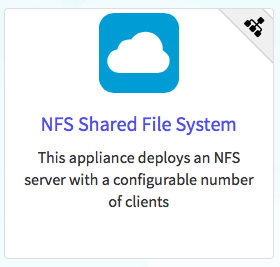
\includegraphics[width=0.5\columnwidth]{images/chameleon/NFS.png}

\section{How do I deploy a complex
appliance?}\label{how-do-i-deploy-a-complex-appliance}

We will explain how to launch a complex appliance based on our
\href{https://www.chameleoncloud.org/appliances/25/}{NFS share
appliance}. To launch a complex appliance, you only need to follow these
steps:

\begin{enumerate}
\item
  Create a lease: use the OpenStack web interface (choose between CHI@UC
  or CHI@TACC) to create a lease. To launch our NFS appliance, reserve
  at least three compute nodes (the strict minimum is two nodes but we
  will use three in this example and later ones).
\item
  Go to the \href{https://www.chameleoncloud.org/appliances/}{Appliance
  Catalog} and identify the appliance you want to launch. In our case
  you can go straight to the
  \href{https://www.chameleoncloud.org/appliances/25/}{NFS
  share~appliance}; click on it to open its details page. You will see a
  ``Launch'' button and a ``Get Template'' button. Follow the ``Get
  Template'' link and copy its url to the clipboard --~you will need it
  in the following steps.
\item
  Click on the ``Launch Complex Appliance at CHI@TACC'' or ``Launch
  Complex Appliance at CHI@UC'' button depending on where your
  reservation was created.
\end{enumerate}

This will take you to the Stacks page within the Orchestration menu.
This page will show the current list of stacks, with controls to manage
them and create new ones. Since we haven't launched any yet, this list
will be empty for now.

We will now create a new stack, which corresponds to the launch of a
template. Click on Launch Stack on the top right. A window will pop up
like below:

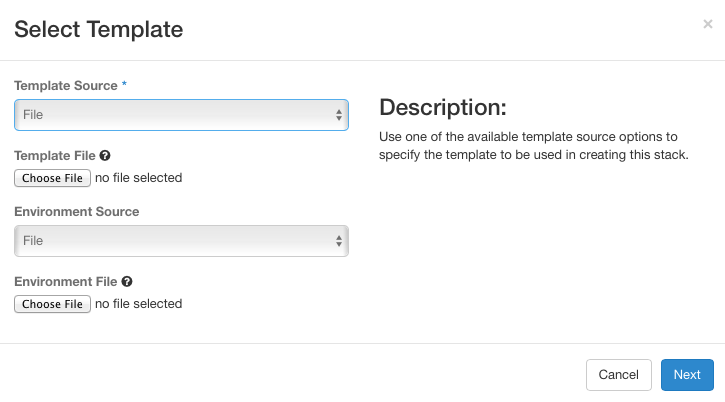
\includegraphics[width=\columnwidth]{images/chameleon/Launch-Stack.png}

We will deploy the NFS appliance described earlier; it will consist of a
server node and two client nodes. Change the template source field to
URL, and paste the URL of the
\href{https://www.chameleoncloud.org/appliances/api/appliances/25/template}{NFS
share~template} (if you don't have it in your clipboard anymore you will
need to go back to the appliance and get it by clicking on ``Get
template'' again).

Don't change the environment source settings, and click ``Next''.

The next screen allows your to enter input values to your Heat template.
Choose a name for your stack (e.g. my-nfs-cluster). Ignore the
``Creation Timeout'' and ``Rollback On Failure'' settings. You also need
to enter your Chameleon password. Then, you need to select a value for
the three parameters of the template: for key\_name, choose your SSH key
pair (this key pair will authorize access on each deployed instances,
both server and client). For nfs\_client\_count, change the default
value of 1 to 2. For reservation\_id, choose your reservation created
earlier. Finally, click ``Launch''.

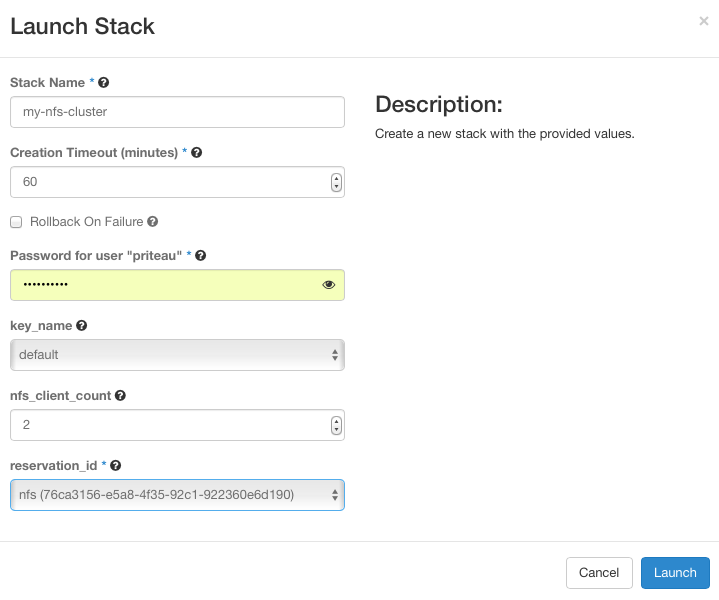
\includegraphics[width=\columnwidth]{images/chameleon/Launch-NFS-Stack.png}

Your stack should be in status ``Create In Progress'' for several
minutes while it first launches the NFS server instance, followed by the
NFS client instances.

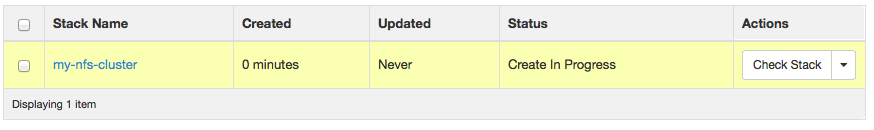
\includegraphics[width=\columnwidth]{images/chameleon/Create-In-Progress_zPgOjo4.png}

It will then move to the status ``Create Complete''.

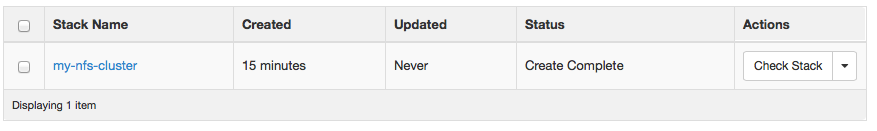
\includegraphics[width=\columnwidth]{images/chameleon/Create-Complete_XkoWhlj.png}

You can click on the stack name to get more details, including a
visualization of the deployed resources, as pictured below. The single
machine inside a circle represents the NFS server instance. The rack of
machine represents the group of NFS client instances (in this case, a
group composed of two instances). The server's floating IP (the public
IP assigned to a resource) is represented by an IP in a circle; an~IP in
a circle is also used to represent the association of the IP with~the
NFS server instance (not the greatest idea to use the same symbol for
both the IP and the association -- we agree but can't do much about it
at the moment). Blow off some steam by dragging the visualization across
the screen, it can be rather fun!

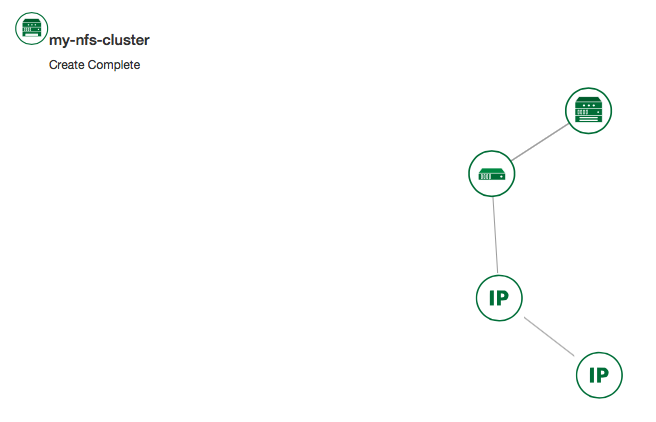
\includegraphics[width=\columnwidth]{images/chameleon/Stack-visualization.png}

You can now ssh to the server using the floating IP just as you do with
regular instances (use the cc account). The client does not have a
floating IP attached to it (as per the visualization above) but you can
connect to it via the server node with the client's private IP (connect
to the server with \texttt{ssh\ -A}~to enable the SSH agent forwarding
after loading your key to your SSH agent
with~\texttt{ssh-add\ \textless{}path-to-your-key\textgreater{}}).

You can find out the information about the IPs and other things if you
click the ``Overview'' tab and look in the ``Outputs'' section. Under
the ``Resources'' tab you will see the resources described above (the
server, clients, server's public/floating IP, and its the association)
and information about them. In the ``Events'' tab you will see
information about the history of the deployment so far. In Template you
will see the template that was used to deploy this stack.

\section{What is inside a Heat
template?}\label{what-is-inside-a-heat-template}

The NFS share appliance deploys:

\begin{itemize}
\item
  an NFS server instance, that exports the directory /exports/example to
  any instance running on Chameleon bare-metal,
\item
  one or several NFS client instances, which configure /etc/fstab to
  mount this NFS share to /mnt (and can subsequently read from and write
  to it).
\end{itemize}

This template is reproduced further below, and includes inline comments
starting with the \# character. There are three main sections:

\begin{itemize}
\item
  resources,
\item
  parameters,
\item
  outputs.
\end{itemize}

The resources section is the most important part of the template: it
defines which OpenStack resources to create and configure. Inside this
section you can see four resources defined:

\begin{itemize}
\item
  nfs\_server\_floating\_ip
\item
  nfs\_server~
\item
  nfs\_server\_ip\_association
\item
  nfs\_clients
\end{itemize}

The first resource, nfs\_server\_floating\_ip, creates a floating IP on
the ext-net public network. It is not attached to any instance yet.

The second resource, nfs\_server, creates the NFS server instance (an
instance is defined with the type \texttt{OS::Nova::Server} in Heat). It
is a bare-metal instance (\texttt{flavor:\ baremetal}) using the
CC-CentOS7 image and connected to the private network named sharednet1.
We set the keypair to use the value of the parameter defined earlier,
using the \texttt{get\_param} function. Similarly, the reservation to
use is passed to the scheduler. Finally, a user-data script is given to
the instance, which configures it as an NFS server exporting
/exports/example to Chameleon instances.

The nfs\_server\_ip\_association resource associates the floating IP
created earlier with the NFS server instance.

Finally, the nfs\_clients resource defines a resource group containing
instance configured to be NFS clients and mount the directory exported
by the NFS server defined earlier. The IP of the NFS server is gathered
using the \texttt{get\_attr} function, and placed into user-data using
the \texttt{str\_replace} function.

Parameters all have the same data structure: each one has a name
(\texttt{key\_name} or \texttt{reservation\_id} in this case), a data
type (number or string), a comment field called description, optionally
a default value, and a list of constraints (in this case only one per
parameter). Constraints tell Heat to match a parameter to a specific
type of OpenStack resource. Complex appliances on Chameleon require
users to customize at least the key pair name and reservation ID, and
will generally provide additional parameters to customize other
properties of the cluster, such as its size, as in this example.

Outputs are declared similarly to parameters: they each have a name, an
optional~description, and a value. They allow to return information from
the~stack to the user.

\begin{footnotesize}
\begin{verbatim}
# This describes what is deployed by this template.
description: NFS server and clients deployed with Heat on Chameleon

# This defines the minimum Heat version required by this template.
heat_template_version: 2015-10-15

# The resources section defines what OpenStack resources are to be deployed and
# how they should be configured.
resources:
  nfs_server_floating_ip:
    type: OS::Nova::FloatingIP
    properties:
      pool: ext-net

  nfs_server:
    type: OS::Nova::Server
    properties:
      flavor: baremetal
      image: CC-CentOS7
      key_name: { get_param: key_name }
      networks:
         - network: sharednet1
      scheduler_hints: { reservation: { get_param: reservation_id } }
      user_data: |
        #!/bin/bash
        yum install -y nfs-utils
        mkdir -p /exports/example
        chown -R cc:cc /exports
        echo '/exports/example 10.140.80.0/22(rw,async) 10.40.0.0/23(rw,async)' >> /etc/exports
        systemctl enable rpcbind && systemctl start rpcbind
        systemctl enable nfs-server && systemctl start nfs-server

  nfs_server_ip_association:
    type: OS::Nova::FloatingIPAssociation
    properties:
      floating_ip: { get_resource: nfs_server_floating_ip }
      server_id: { get_resource: nfs_server }

  nfs_clients:
    type: OS::Heat::ResourceGroup
    properties:
      count: { get_param: nfs_client_count }
      resource_def:
        type: OS::Nova::Server
        properties:
          flavor: baremetal
          image: CC-CentOS7
          key_name: { get_param: key_name }
          networks:
             - network: sharednet1
          scheduler_hints: { reservation: { get_param: reservation_id } }
          user_data:
            str_replace:
              template: |
                #!/bin/bash
                yum install -y nfs-utils
                echo "$nfs_server_ip:/exports/example    /mnt/    nfs" > /etc/fstab
                mount -a
              params:
                $nfs_server_ip: { get_attr: [nfs_server, first_address] }

# The parameters section gathers configuration from the user.
parameters:
  nfs_client_count:
    type: number
    description: Number of NFS client instances
    default: 1
    constraints:
      - range: { min: 1 }
        description: There must be at least one client.
  key_name:
    type: string
    description: Name of a KeyPair to enable SSH access to the instance
    default: default
    constraints:
    - custom_constraint: nova.keypair
  reservation_id:
    type: string
    description: ID of the Blazar reservation to use for launching instances.
    constraints:
    - custom_constraint: blazar.reservation

outputs:
  server_ip:
    description: Public IP address of the NFS server
    value: { get_attr: [nfs_server_floating_ip, ip] }
  client_ips:
    description: Private IP addresses of the NFS clients
    value: { get_attr: [nfs_clients, first_address] }
\end{verbatim}
\end{footnotesize}

\section{Customizing an existing
template}\label{customizing-an-existing-template}

Customizing an existing template is a good way to start developing your
own. We will use a simpler template than the previous example to start
with: it is
the~\href{https://www.chameleoncloud.org/appliances/26/}{Hello World
complex appliance}.

First, delete the stack you launched, because we will need all three
nodes to be free. To do this, go back to the Project \textgreater{}
Orchestration \textgreater{} Stacks page, select your stack, and then
click on the red ``Delete Stacks'' button. You will be asked to confirm,
so click on the blue~``Delete Stacks'' button.

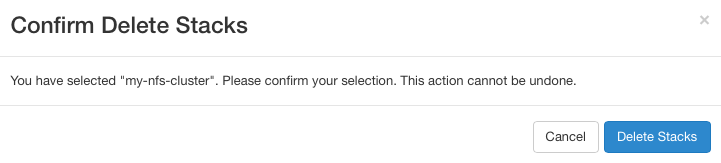
\includegraphics[width=\columnwidth]{images/chameleon/Delete-Stacks.png}

The template for the
\href{https://www.chameleoncloud.org/appliances/26/}{Hello World complex
appliance}~is~reproduced below. It is similar to the NFS share
appliance, except that it deploys only a single client. You can see that
it has four resources defined:

\begin{itemize}
\item
  nfs\_server\_floating\_ip
\item
  nfs\_server
\item
  nfs\_server\_ip\_association
\item
  nfs\_client
\end{itemize}

The nfs\_client instance mounts the NFS directory shared by the
nfs\_server instance, just like in our earlier example.

\begin{footnotesize}
\begin{verbatim}
# This describes what is deployed by this template.
description: NFS server and client deployed with Heat on Chameleon

# This defines the minimum Heat version required by this template.
heat_template_version: 2015-10-15

# The resources section defines what OpenStack resources are to be deployed and
# how they should be configured.
resources:
  nfs_server_floating_ip:
    type: OS::Nova::FloatingIP
    properties:
      pool: ext-net

  nfs_server:
    type: OS::Nova::Server
    properties:
      flavor: baremetal
      image: CC-CentOS7
      key_name: { get_param: key_name }
      networks:
         - network: sharednet1
      scheduler_hints: { reservation: { get_param: reservation_id } }
      user_data: |
        #!/bin/bash
        yum install -y nfs-utils
        mkdir -p /exports/example
        chown -R cc:cc /exports
        echo '/exports/example 10.140.80.0/22(rw,async) 10.40.0.0/23(rw,async)' >> /etc/exports
        systemctl enable rpcbind && systemctl start rpcbind
        systemctl enable nfs-server && systemctl start nfs-server

  nfs_server_ip_association:
    type: OS::Nova::FloatingIPAssociation
    properties:
      floating_ip: { get_resource: nfs_server_floating_ip }
      server_id: { get_resource: nfs_server }

  nfs_client:
    type: OS::Nova::Server
    properties:
      flavor: baremetal
      image: CC-CentOS7
      key_name: { get_param: key_name }
      networks:
         - network: sharednet1
      scheduler_hints: { reservation: { get_param: reservation_id } }
      user_data:
        str_replace:
          template: |
            #!/bin/bash
            yum install -y nfs-utils
            echo "$nfs_server_ip:/exports/example    /mnt/    nfs" > /etc/fstab
            mount -a
          params:
            $nfs_server_ip: { get_attr: [nfs_server, first_address] }

# The parameters section gathers configuration from the user.
parameters:
  key_name:
    type: string
    description: Name of a KeyPair to enable SSH access to the instance
    default: default
    constraints:
    - custom_constraint: nova.keypair
  reservation_id:
    type: string
    description: ID of the Blazar reservation to use for launching instances.
    constraints:
    - custom_constraint: blazar.reservation
\end{verbatim}
\end{footnotesize}

Download this template from the
\href{https://www.chameleoncloud.org/appliances/26/}{Hello World complex
appliance details page} to your local machine, and open it in your
favorite text editor.

We will customize~the template to add a second NFS~client by creating a
new resource called another\_nfs\_client. Add the following text to your
template inside the resources section.~Make sure to respect the level of
indentation, which is important in YAML.

\begin{footnotesize}
\begin{verbatim}
  another_nfs_client:
    type: OS::Nova::Server
    properties:
      flavor: baremetal
      image: CC-CentOS7
      key_name: { get_param: key_name }
      networks:
         - network: sharednet1
      scheduler_hints: { reservation: { get_param: reservation_id } }
      user_data:
        str_replace:
          template: |
            #!/bin/bash
            yum install -y nfs-utils
            echo "$nfs_server_ip:/exports/example    /mnt/    nfs" > /etc/fstab
            mount -a
          params:
            $nfs_server_ip: { get_attr: [nfs_server, first_address] }
\end{verbatim}
\end{footnotesize}

Now, launch a new~stack~with this~template. Since the customized
template is only on your computer and cannot be addressed by a URL, use
the ``Direct Input'' method instead and copy/paste the content of the
customized template.~The resulting topology view is shown below:~as you
can see, the two client instances are shown separately since each one is
defined as a separate resource in the template.

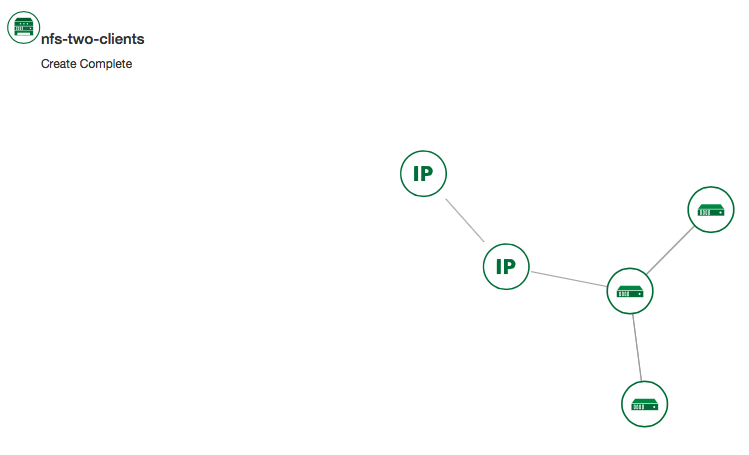
\includegraphics[width=\columnwidth]{images/chameleon/NFS-Two-Clients_lFGgizN.png}

You may have realized~already that while adding just one additional
client instance~was easy, launching more of them would require to copy /
paste blocks of YAML many times while ensuring that the total count is
correct. This would be easy to get wrong, especially when dealing with
tens or hundreds of instances.

So instead, we leverage another construct from Heat: resource groups.
Resource groups allow to define one kind of resource and request it to
be created any~number of times.

Remove the nfs\_client and another\_client resources from your
customized template, and replace them with the following:

\begin{footnotesize}
\begin{verbatim}
  nfs_clients:
    type: OS::Heat::ResourceGroup
    properties:
      count: 2
      resource_def:
        type: OS::Nova::Server
        properties:
          flavor: baremetal
          image: CC-CentOS7
          key_name: { get_param: key_name }
          networks:
             - network: sharednet1
          scheduler_hints: { reservation: { get_param: reservation_id } }
          user_data:
            str_replace:
              template: |
                #!/bin/bash
                yum install -y nfs-utils
                echo "$nfs_server_ip:/exports/example    /mnt/    nfs" > /etc/fstab
                mount -a
              params:
                $nfs_server_ip: { get_attr: [nfs_server, first_address] }
\end{verbatim}
\end{footnotesize}

A resource group is configured with a properties field, containing the
definition of the resource to launch (\texttt{resource\_def}) and the
number of resources to launch (\texttt{count}). Once launched, you will
notice that the topology view groups all client instances under a single
Resource Group icon. We use the same \texttt{resource\_def} than when
defining separate instances earlier.

Another way we can customize this template is by adding outputs to the
template. Outputs allow a Heat template to return data to the user. This
can be useful to return values like IP addresses or credentials that the
user must know to use the system.

We will create an output returning the floating IP address used by the
NFS server. We define an outputs section, and one output with the name
\texttt{server\_ip} and a description. The value of the output is
gathered using the \texttt{get\_attr} function which obtains the IP
address of the server instance.

\begin{footnotesize}
\begin{verbatim}
outputs:
  server_ip:
    description: Public IP address of the NFS server
    value: { get_attr: [nfs_server_floating_ip, ip] }
\end{verbatim}
\end{footnotesize}

You can get outputs in the ``Overview'' tab of the Stack~Details page.
If you want to use~the command line, install \texttt{python-heatclient}
and use~the \texttt{heat\ output-list} and \texttt{heat\ output-show}
commands, or get a full list in the information returned by
\texttt{heat\ stack-show}.

Multiple outputs can be defined in the outputs section. Each of them
needs to have a unique name. For example, we can add another output to
list the private IPs assigned to client instances:

\begin{footnotesize}
\begin{verbatim}
  client_ips:
    description: Private IP addresses of the NFS clients
    value: { get_attr: [nfs_clients, first_address] }
\end{verbatim}
\end{footnotesize}

The image below shows the resulting outputs as viewed from the web
interface. Of course IP addresses will be specific to each deployment.

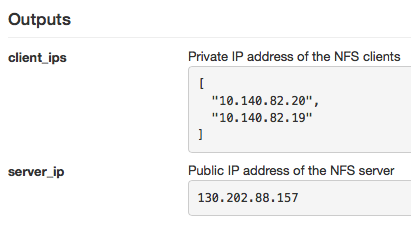
\includegraphics[width=0.5\columnwidth]{images/chameleon/Outputs.png}

Finally, we can add a new parameter to replace the hardcoded number of
client instances by a value passed to the template. Add the following
text to the parameters section:

\begin{footnotesize}
\begin{verbatim}
  nfs_client_count:
    type: number
    description: Number of NFS client instances
    default: 1
    constraints:
      - range: { min: 1 }
        description: There must be at least one client.
\end{verbatim}
\end{footnotesize}

Inside the resource group definition,
change~\texttt{count:\ 2}~to~\texttt{count:\ \{\ get\_param:\ nfs\_client\_count\ \}}~to
retrieve and use the parameter we just defined. When you launch this
template, you will see that an additional parameter allows you to define
the number of client instances, like in the NFS share~appliance.

At this stage, we have fully recreated the NFS share appliance starting
from the Hello World one! The next section will explain how to write a
new template from scratch.

\section{Writing a new template}\label{writing-a-new-template}

You may want to write a whole new template, rather than customizing an
existing one. Each template should follow the same layout and be
composed of the following sections:

\begin{itemize}
\item
  Heat template version
\item
  Description
\item
  Resources
\item
  Parameters
\item
  Outputs
\end{itemize}

\subsection{Heat template version}\label{heat-template-version}

Each Heat template has to include the heat\_template\_version key with a
valid version of HOT (Heat Orchestration Template). Chameleon bare-metal
supports any HOT version up to 2015-10-15, which corresponds to
OpenStack Liberty. The
\href{http://docs.openstack.org/developer/heat/template_guide/hot_spec.html\#hot-spec-template-version}{Heat
documentation}~lists~all available~versions and their features.~We
recommended that you always use the latest supported~version to have
access to all supported features:

\texttt{heat\_template\_version:\ 2015-10-15}

\subsection{Description}\label{description}

While not mandatory, it is good practice to describe what ~is deployed
and configured by your template. It can be on a single line:

\begin{footnotesize}
\begin{verbatim}
description: This describes what this Heat template deploys on Chameleon.
\end{verbatim}
\end{footnotesize}

If a longer description is needed, you can provide multi-line text in
YAML, for example:

\begin{footnotesize}
\begin{verbatim}
description: >
  This describes what this Heat
  template deploys on Chameleon.
\end{verbatim}
\end{footnotesize}

\subsection{Resources}\label{resources}

The resources section is required and must contain at least one resource
definition. A
\href{http://docs.openstack.org/developer/heat/template_guide/openstack.html}{complete
list of resources types known to Heat} is available.

However, only a subset of them are supported by Chameleon, and some are
limited to administrative use. We recommend that you only use:

\begin{itemize}
\item
  OS::Glance::Image
\item
  OS::Heat::ResourceGroup
\item
  OS::Heat::SoftwareConfig
\item
  OS::Heat::SoftwareDeployment
\item
  OS::Heat::SoftwareDeploymentGroup
\item
  OS::Neutron::FloatingIP
\item
  OS::Neutron::FloatingIPAssociation
\item
  OS::Neutron::Port (advanced users only)
\item
  OS::Nova::Keypair
\item
  OS::Nova::Server
\end{itemize}

If you know of another resource that you would like to use and think it
should be supported by the OpenStack services on Chameleon bare-metal,
please let us know via our help desk.

\subsection{Parameters}\label{parameters}

Parameters allow users to customize the template with necessary or
optional values. For example, they can customize which Chameleon
appliance they want to deploy, or which key pair to install. Default
values can be provided with the \texttt{default} key, as well as
constraints to ensure that only valid OpenStack resources can be
selected. For example, \texttt{custom\_constraint:\ glance.image}
restricts the image selection to an available OpenStack image, while
providing a pre-filled selection box in the web interface.
\href{http://docs.openstack.org/developer/heat/template_guide/hot_spec.html\#parameter-constraints}{More
details about constraints}~are available in the Heat documentation.

\subsection{Outputs}\label{outputs}

Outputs allow template to give information from the deployment to users.
This can include usernames, passwords, IP addresses, hostnames, paths,
etc. The outputs declaration is using the following format:

\begin{footnotesize}
\begin{verbatim}
outputs:
  first_output_name:
    description: Description of the first output
    value: first_output_value
  second_output_name:
    description: Description of the second output
    value: second_output_value
\end{verbatim}
\end{footnotesize}

Generally values will be calls to get\_attr, get\_param, or some other
function to get information from parameters or resources deployed by the
template and return them in the proper format to the user.

\section{Sharing new complex
appliances}\label{sharing-new-complex-appliances}

If you have written your own complex appliances
or~substantially~customized an existing one, we would love if you shared
them with our user community!

The process is very similar to regular appliances: log into the
Chameleon portal, go to the
\href{https://www.chameleoncloud.org/appliances/}{appliance catalog},
and click on the button in the top-right corner: ``Add an appliance''
(you need to be logged in to see it).


\includegraphics[width=0.25\columnwidth]{images/chameleon/Add-an-appliance.png}

You will be prompted to enter a name, description, and documentation.
Instead of providing appliance IDs, copy your template to the dedicated
field. Finally, share your contact information and assign a version
string to your appliance. Once submitted, your appliance will be
reviewed. We will get in touch if a change is needed, but if it's all
good we will publish it right away!

\section{Advanced topics}\label{advanced-topics}

\subsection{All-to-all information
exchange}\label{all-to-all-information-exchange}

The previous examples have all used user-data scripts to provide
instances with contextualization information. While it is easy to use,
this contextualization method has a major drawback: because it is given
to the instance as part of its launch request, it cannot use any context
information that is not yet known at this time.

In practice, this means that in a client-server deployment, only one of
these pattern will be possible:

\begin{itemize}
\item
  The server has to be deployed first, and once it is deployed, the
  clients can be launched and contextualized with information from the
  server. The server won't know about the clients unless there is a
  mechanism (not managed by Heat) for the client to contact the server.
\item
  The clients have to be deployed first, and once they are deployed, the
  server can be launched and contextualized with information from the
  clients. The clients won't know about the server unless there is a
  mechanism (not managed by Heat) for the server to contact the clients.
\end{itemize}

This limitation was already apparent in our NFS share~appliance: this is
why the server instance exports the file system to all bare-metal
instances on Chameleon, because it doesn't know which specific IP
addresses are allocated to the clients.

This limitation is even more important if the deployment is not
hierarchical, i.e. all instances need to know about all others. For
example, a cluster with IP and hostnames populated in /etc/hosts
required each instance to be known by every other instance.

This section presents a more advanced form of contextualization that can
perform this kind of information exchange. This is implemented by Heat
agents running inside instances and communicating with the Heat service
to send and receive information. This means you will need to use an
image bundling these agents. Currently, our CC-CentOS7 appliance and its
CUDA version are the only ones supporting this mode of
contextualization. If you build your own images using the
\href{https://github.com/ChameleonCloud/CC-CentOS7}{CC-CentOS7 appliance
builder}, you will automatically have these agents installed.

This contextualization is performed with several Heat resources:

\begin{itemize}
\item
  \texttt{OS::Heat::SoftwareConfig}.~This resource describes code to run
  on an instance. It can be configured with inputs and provide outputs.
\item
  \texttt{OS::Heat::SoftwareDeployment}. This resource applies a
  SoftwareConfig to a specific instance.
\item
  \texttt{OS::Heat::SoftwareDeploymentGroup}. This resource applies a
  SoftwareConfig to a specific group of instances.
\end{itemize}

The template below illustrates how it works. It launches a group of
instances that will automatically populates their /etc/hosts file with
IP and hostnames from other instances in the deployment.

\begin{footnotesize}
\begin{verbatim}
heat_template_version: 2015-10-15

description: >
  This template demonstrates how to exchange hostnames and IP addresses to populate /etc/hosts.

parameters:
  flavor:
    type: string
    default: baremetal
    constraints:
    - custom_constraint: nova.flavor
  image:
    type: string
    default: CC-CentOS7
    constraints:
    - custom_constraint: glance.image
  key_name:
    type: string
    default: default
    constraints:
    - custom_constraint: nova.keypair
  instance_count:
    type: number
    default: 2
  reservation_id:
    type: string
    description: ID of the Blazar reservation to use for launching instances.
    constraints:
    - custom_constraint: blazar.reservation

resources:
  export_hosts:
    type: OS::Heat::SoftwareConfig
    properties:
      outputs:
        - name: hosts
      group: script
      config: |
        #!/bin/sh
        (echo -n $(facter ipaddress); echo -n ' '; echo $(facter hostname)) > ${heat_outputs_path}.hosts

  export_hosts_sdg:
    type: OS::Heat::SoftwareDeploymentGroup
    properties:
      config: { get_resource: export_hosts }
      servers: { get_attr: [server_group, refs_map] }
      signal_transport: HEAT_SIGNAL

  populate_hosts:
    type: OS::Heat::SoftwareConfig
    properties:
      inputs:
        - name: hosts
      group: script
      config: |
        #!/usr/bin/env python
        import ast
        import os
        import string
        import subprocess
        hosts = os.getenv('hosts')
        if hosts is not None:
            hosts = ast.literal_eval(string.replace(hosts, '\n', '\\n'))
        with open('/etc/hosts', 'a') as hosts_file:
          for ip_host in hosts.values():
              hosts_file.write(ip_host.rstrip() + '\n')

  populate_hosts_sdg:
    type: OS::Heat::SoftwareDeploymentGroup
    depends_on: export_hosts_sdg
    properties:
      config: { get_resource: populate_hosts }
      servers: { get_attr: [server_group, refs_map] }
      signal_transport: HEAT_SIGNAL
      input_values:
        hosts: { get_attr: [ export_hosts_sdg, hosts ] }

  server_group:
    type: OS::Heat::ResourceGroup
    properties:
      count: { get_param: instance_count }
      resource_def:
        type: OS::Nova::Server
        properties:
          flavor: { get_param: flavor }
          image: { get_param: image }
          key_name: { get_param: key_name }
          networks:
             - network: sharednet1
          scheduler_hints: { reservation: { get_param: reservation_id } }
          user_data_format: SOFTWARE_CONFIG
          software_config_transport: POLL_SERVER_HEAT

outputs:
  deployment_results:
    value: { get_attr: [export_hosts_sdg, hosts] }
\end{verbatim}
\end{footnotesize}

There are two SoftwareConfig resources.

The first SoftwareConfig, export\_hosts, uses the facter tool to extract
IP address and hostname into a single line (in the format expected for
/etc/hosts) and writes it to a special path
(\$\{heat\_outputs\_path\}.hosts). This prompts Heat to assign the
content of this file to the output with the name hosts.

The second SoftwareConfig, populate\_hosts, takes as input a variable
named hosts, and applies a script that reads the variable from the
environment, parses it with ast.literal\_eval (as it is formatted as a
Python dict), and writes each value of the dictionary to /etc/hosts.

The SoftwareDeploymentGroup resources export\_hosts\_sdg and
populate\_hosts\_sdg apply each SoftwareConfig to the instance
ResourceGroup with the correct configuration.

Finally, the instance ResourceGroup is configured so that each instance
uses the following contextualization method instead of a user-data
script:

\begin{footnotesize}
\begin{verbatim}
          user_data_format: SOFTWARE_CONFIG
          software_config_transport: POLL_SERVER_HEAT
\end{verbatim}
\end{footnotesize}

You can follow the same template pattern to configure your own
deployment requiring all-to-all information exchange.


